\section{Grundlagen und Stand der Technik}

Salvaris beschreibt das \textit{Machine Learning} (ML) als einen Zweig der Computerwissenschaften, bei dem Computern beigebracht wird anhand von Trainingsdaten Entscheidungen zu treffen. Typische Anwendungsgebiete des ML sind Klassifikation, Regression und Clustering. Das \textit{Deep Learning} (DL) ist ein Teilgebiet des ML (Abb. \ref{dlmlunterschied}) bei dem besonders komplexe neuronale Netze mit vielen Schichten und Neuronen Verwendung finden. Eine weitere wesentliche Abgrenzung stellt die Merkmalsextraktion dar. Also die Extraktion der Eigenschaften eines Objekts, die ausschlaggebend für etwaige Klassenzugehörigkeiten sind. Diese entscheidenden Merkmale müssen dem DL-Modell nicht vorgegeben werden, sondern werden von dem Algorithmus selbst gefunden. Dieser Umstand stellt mit die größten Herausforderungen aber auch Chancen beim DL dar \cite[S.32-47]{dlazure2019}.  Im Folgenden werden nur die für die vorliegende Arbeit besonders relevanten und speziell angepassten Methoden und Aspekte des DL erläutert. Für weiterführende grundlegende Informationen zum Beispiel zu Neuronen, Schichttypen, Aktivierungsfunktionen und zum Gradientenabstiegsverfahren wird auf \cite{dlbook2018} verwiesen. 
\begin{figure}[!h]
  \centering
  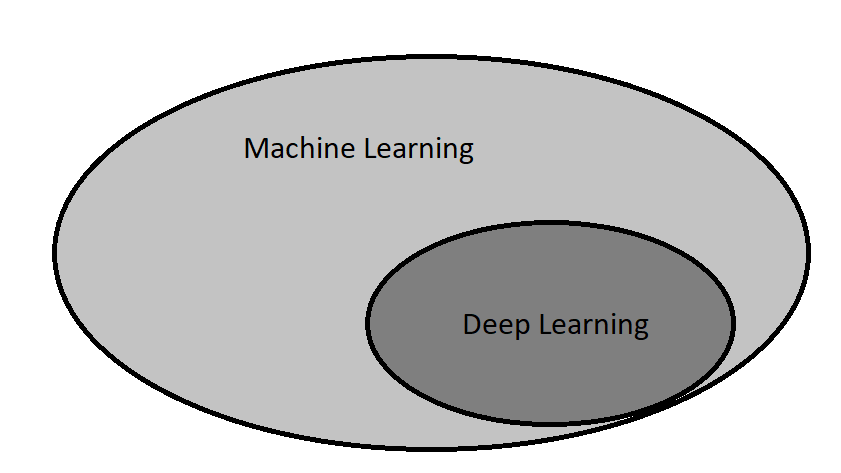
\includegraphics[width=8cm]{mldlunterschied.png}
  \caption{Abgrenzung Deep Learning zu Machine Learning}
  \label{dlmlunterschied}
\end{figure}

\subsection{Convolutional Neural Networks}

\textit{Convolutional Neural Networks} (CNN) sind eine spezielle Art von neuronalen Netzen, die sich für das verarbeiten von gitterartig beschaffenen Daten eignen. Hierzu zählen zum Beispiel auch Bilddaten, deren Pixelraster sich als Gitter oder Matrix interpretieren lassen. Ein typisches CNN besteht dabei aus einem oder mehreren Paaren von \textit{Convolutional}- und \textit{Pooling-Layern}, gefolgt von einem oder mehreren \textit{Fully-Connected-Layern}. Die Folgenden Darstellungen richten sich im wesentlichen nach Goodfellow \cite[S.326-366]{Goodfellow-et-al-2016}
\paragraph{Convolutional Layer}
Bei einem \textit{Convolutional Layer} wird schrittweise ein Filterkernel $K$ über eine Eingabematrix $I$ mit den Dimensionen $n$ und $m$ bewegt (Abb. \ref{cnns}). Der Input der folgenden Neuronen $S(i,j)$ berechnet sich dann aus einer Faltungsoperation der jeweils übereinanderliegenden Kernel- und Bildelemente (Gleichung \ref{convolution}). 
\begin{equation}\label{convolution}
	S(i,j)=(I\ast K)(i,j)=\sum_{n}\sum_{n} I(i-m,j-n)K(m,n)
\end{equation}
Der so berechnete Input eines Neurons wird anschließend abhängig von der verwendeten Aktivierungsfunkton in den Output verwandelt. Zu bemerken ist, dass alle Neuronen eines \textit{Convolutional Layers} die gleichen Gewichte haben (sog. \textit{Parameter Sharing}). Dadurch ist es möglich Speicher gegenüber anderen Netzstrukturen einzusparen, die häufig eine große Gewichtungsmatrix verwenden. Ein weiterer großer Vorteil sind die sog. \textit{Sparse Interarctions}. Durch die Verwendung eines Filterkernels der meist nur einen Bruchteil der Größe des zu analysierenden Bildes aufweist, werden nur die Features extrahiert, die wirklich entscheidend sind für die Zugehörigkeit zu einer Klasse. Dies führt ebenso zu einer weiteren Speicher- und Performanzoptimierung.
\begin{figure}[h!]
  \centering
  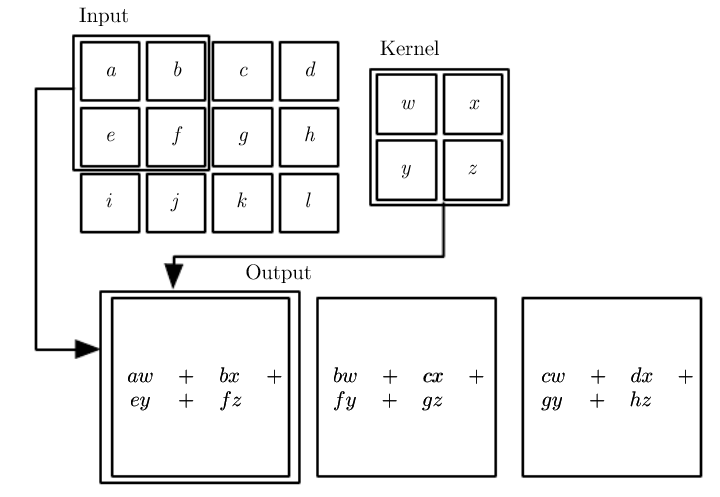
\includegraphics[width=12cm]{cnn_prinzip.png}
  \caption{Prinzip eines Convolutional Layers \cite[S.330]{Goodfellow-et-al-2016}}
  \label{cnns}
\end{figure}
\paragraph{Pooling Layer}

\textit{Pooling Layer} sorgen dafür, dass Features einer Klasse in einem Bild nahezu ortsinvariant gelernt werden können. Ein weitverbreitetes Pooling Verfahren ist das sog. $2X2$ \textit{Max-Pooling}, bei dem aus jedem $2X2$ Quadrat der Neuronen des \textit{Convolutional-Layers} nur das aktivste Neuron an die nächste Schicht weitergeleitet wird. Abbildung \ref{poolinglayer} verdeutlicht dieses Funktionsprinzip. Es werden von den jeweils benachbarten Neuronen nur die mit den höchsten Gewichten an die nächste Schicht durchgeschaltet.
\begin{figure}[!h]
  \centering
  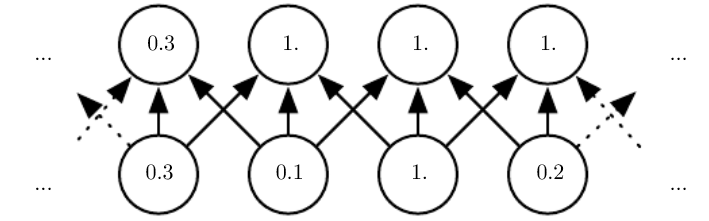
\includegraphics[width=12cm]{pooling_layer.png}
  \caption{Prinzip eines Pooling Layers \cite[S.337]{Goodfellow-et-al-2016}}
  \label{poolinglayer}
\end{figure} 
\FloatBarrier

\paragraph{Fully Connected Layer}

\textit{Fully-Connected-Layer} oder in \textit{Keras} sog. \textit{Dense-Layer} stellen einen Schichtentyp dar, bei dem jedes Neuron mit jeweils jedem Neuron der vorigen Schicht verschaltet ist. Es ist so möglich, die Ausgaben des letzten \textit{Pooling-Layers} über ein oder mehrere \textit{Fully-Connected-Layer} mithilfe von Aktivierungsfunktionen zum Beispiel in eine Wahrscheinlichkeitsverteilung der Klassenzugehörigkeit zu überführen. Die Anzahl Neuronen in der letzten Schicht entspricht dann der Anzahl zu lernender Klassen oder auch der Anzahl vorherzusagender Features.

\subsection{Loss-Funktionen und Metriken}

DL Netze optimieren ihre Gewichte und Neuronenaktivitäten während des Trainings selbst durch einen Vergleich der geschätzten Ergebnisse $y_{pred}$ mit den entsprechenden Zielgrößen $y_{target}$. Dies geschieht über sog. \textit{Loss-Functions}. Dabei zeigen diese Funktionen bei großen Abweichung von den Zielwertebereichen typischerweise auch hohe Werte \cite[S.271-279]{Goodfellow-et-al-2016}. Ein weit verbreitetes Beispiel hierfür ist der mittlere quadratische Fehler (\textit{Mean-Squared-Error (MSE)}), der häufig als Maß zur Evaluation des Trainingserfolges eingesetzt wird. Der MSE berechnet sich entsprechend Gleichung \ref{mse}. Die MSE-Loss-Funktion wird auch als L2-Loss bezeichnet. Diese Möglichkeit zur Beurteilung des Erfolges eines DL-Modells wird in Keras auch als Metrik bezeichnet. Als Metriken werden meist ebenso die beschriebenen Loss-Funktionen verwendet. Metriken haben einen rein informativen Zweck und werden nicht direkt für das Training verwendet \cite{chollet2015keras}. Loss-Funktionen spiegeln so einen entscheidenden Faktor für ein erfolgreiches Training wieder. Dabei sollte je nach Anwendungsfall individuell eine passende und sinnvolle Loss-Funktion zur Validierung gewählt werden. Ein ausführliche Abhandlung hierüber findet sich in \cite{dlbook2018} und \citep{dlazure2019}.
\begin{equation}\label{mse}
	MSE=\sum_{n} \frac{(y_{pred}-y_{target})^2}{n}
\end{equation}

\subsection{Stand der Technik}

In der Literatur werden viele Möglichkeiten zur Objekterkennung mittels DL beschrieben. Laut Zhao haben sich aktuell jedoch drei Hauptverfahren in der Industrie etabliert \cite{Detection2019}. \textit{Fast-Region-Based-CNNs} ermöglichen gute Detektionsergebnisse, sind aber relativ rechenaufwendig \cite{Girshick2015}. Das \textit{You Only Look Once} Modell (YOLO) erreicht eine höhere Performanz bei verbesserter Präzision \cite{Redmon2016}. Ein weiteres Modell zur Lösung des Problems ist das von Liu vorgestellte \textit{Single-Shot-Detection} (SSD) Modell vor. Beim SSD können Performanz und Genauigkeit zu Lasten einer komplexeren Netzarchitektur noch weiter verbessert werden \cite{Liu2016}. Die Gemeinsamkeit aller vorgestellten Modelle besteht in der Verwendung von \textit{Convolutional Layern}.